\begin{figure}[htbp]
\centering
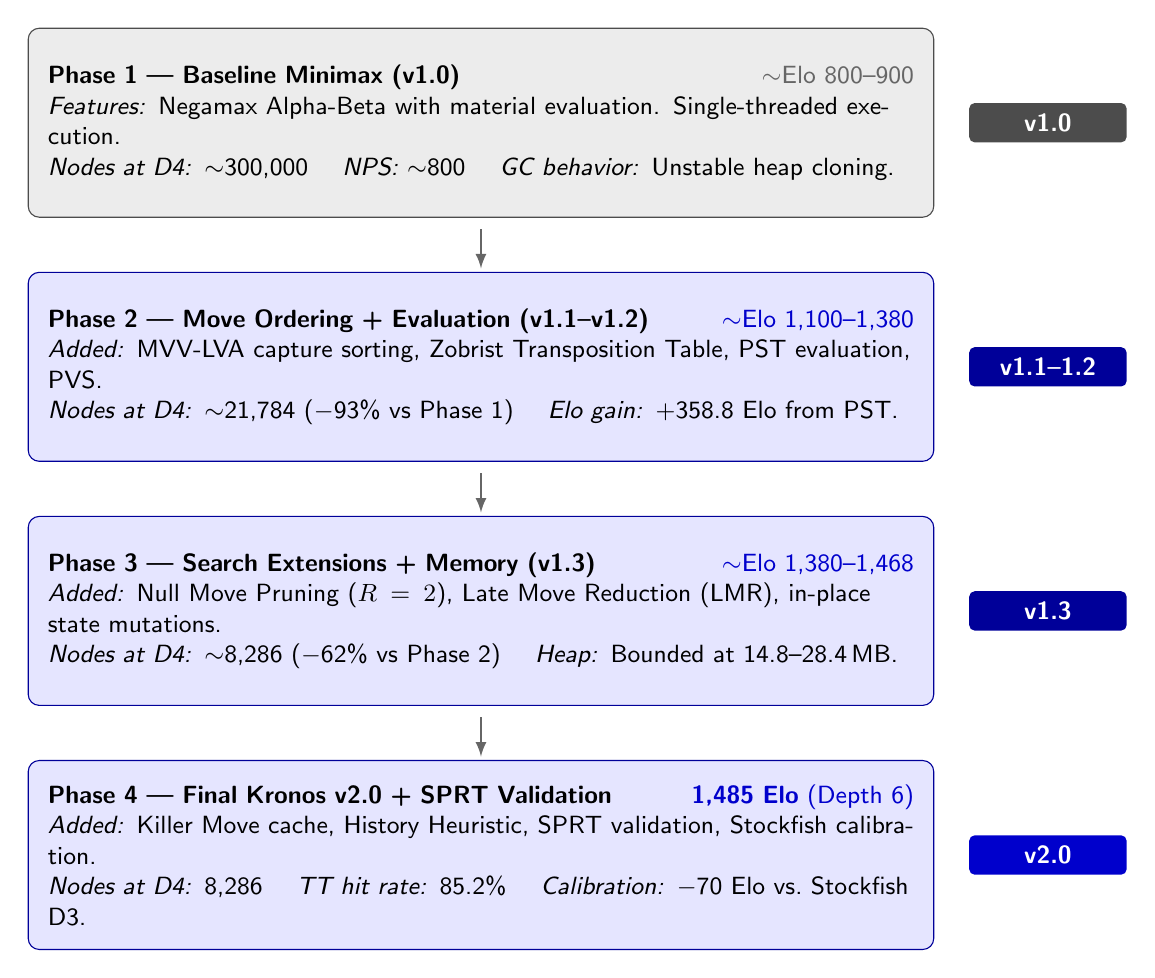
\begin{tikzpicture}[
    node distance=0cm,
    phase/.style={
        draw=blue!60!black, rectangle, rounded corners=4pt,
        minimum width=11.5cm, minimum height=2.4cm,
        text width=11.0cm, align=left,
        fill=blue!10, font=\small\sffamily
    },
    phaseA/.style={phase, fill=gray!15,  draw=gray!60!black},
    phaseB/.style={phase, fill=blue!10,  draw=blue!60!black},
    phaseC/.style={phase, fill=blue!10,  draw=blue!60!black},
    phaseD/.style={phase, fill=blue!10,  draw=blue!60!black},
    arrow/.style={draw, -latex, thick, gray!80!black},
    label/.style={font=\bfseries\small\sffamily, text=white, fill=gray!70, rounded corners=2pt,
                  minimum width=2.0cm, minimum height=0.5cm, align=center}
]

% ===== Phase 1 =====
\node[phaseA] (p1) at (0,0) {%
    \textbf{Phase 1 — Baseline Minimax (v1.0)} \hfill \textcolor{gray!80!black}{$\sim$Elo 800--900}\\
    \textit{Features:} Negamax Alpha-Beta with material evaluation. Single-threaded execution.\\
    \textit{Nodes at D4:} $\sim$300{,}000 \quad \textit{NPS:} $\sim$800 \quad \textit{GC behavior:} Unstable heap cloning.
};

\draw[arrow] (0,-1.35) -- (0,-1.85);

% ===== Phase 2 =====
\node[phaseB] (p2) at (0,-3.1) {%
    \textbf{Phase 2 — Move Ordering + Evaluation (v1.1--v1.2)} \hfill \textcolor{blue!80!black}{$\sim$Elo 1{,}100--1{,}380}\\
    \textit{Added:} MVV-LVA capture sorting, Zobrist Transposition Table, PST evaluation, PVS.\\
    \textit{Nodes at D4:} $\sim$21{,}784 ($-$93\% vs Phase 1) \quad \textit{Elo gain:} $+$358.8 Elo from PST.
};

\draw[arrow] (0,-4.45) -- (0,-4.95);

% ===== Phase 3 =====
\node[phaseC] (p3) at (0,-6.2) {%
    \textbf{Phase 3 — Search Extensions + Memory (v1.3)} \hfill \textcolor{blue!80!black}{$\sim$Elo 1{,}380--1{,}468}\\
    \textit{Added:} Null Move Pruning ($R=2$), Late Move Reduction (LMR), in-place state mutations.\\
    \textit{Nodes at D4:} $\sim$8{,}286 ($-$62\% vs Phase 2) \quad \textit{Heap:} Bounded at 14.8--28.4\,MB.
};

\draw[arrow] (0,-7.55) -- (0,-8.05);

% ===== Phase 4 =====
\node[phaseD] (p4) at (0,-9.3) {%
    \textbf{Phase 4 — Final Kronos v2.0 + SPRT Validation} \hfill \textcolor{blue!80!black}{\textbf{1{,}485 Elo} (Depth 6)}\\
    \textit{Added:} Killer Move cache, History Heuristic, SPRT validation, Stockfish calibration.\\
    \textit{Nodes at D4:} 8{,}286 \quad \textit{TT hit rate:} 85.2\% \quad \textit{Calibration:} $-$70 Elo vs.\ Stockfish D3.
};

% Right-side metric labels
\node[label, fill=gray!60!black]   at (7.2, 0)    {v1.0};
\node[label, fill=blue!60!black]   at (7.2, -3.1) {v1.1--1.2};
\node[label, fill=blue!60!black]   at (7.2, -6.2) {v1.3};
\node[label, fill=blue!80!black]  at (7.2, -9.3) {v2.0};

\end{tikzpicture}
\caption[Kronos Engine Development Progression]{Kronos engine development progression across optimization phases.}
\label{fig:kronos_evolution}
\end{figure}

% Source Material: ENGINE_FEATURE_MATRIX.md, benchmark ablation results
